
%% bare_conf_compsoc.tex
%% V1.4a
%% 2014/09/17
%% by Michael Shell
%% See:
%% http://www.michaelshell.org/
%% for current contact information.
%%
%% This is a skeleton file demonstrating the use of IEEEtran.cls
%% (requires IEEEtran.cls version 1.8s or later) with an IEEE Computer
%% Society conference paper.
%%
%% Support sites:
%% http://www.michaelshell.org/tex/ieeetran/
%% http://www.ctan.org/tex-archive/macros/latex/contrib/IEEEtran/
%% and
%% http://www.ieee.org/

%%*************************************************************************
%% Legal Notice:
%% This code is offered as-is without any warranty either expressed or
%% implied; without even the implied warranty of MERCHANTABILITY or
%% FITNESS FOR A PARTICULAR PURPOSE!
%% User assumes all risk.
%% In no event shall IEEE or any contributor to this code be liable for
%% any damages or losses, including, but not limited to, incidental,
%% consequential, or any other damages, resulting from the use or misuse
%% of any information contained here.
%%
%% All comments are the opinions of their respective authors and are not
%% necessarily endorsed by the IEEE.
%%
%% This work is distributed under the LaTeX Project Public License (LPPL)
%% ( http://www.latex-project.org/ ) version 1.3, and may be freely used,
%% distributed and modified. A copy of the LPPL, version 1.3, is included
%% in the base LaTeX documentation of all distributions of LaTeX released
%% 2003/12/01 or later.
%% Retain all contribution notices and credits.
%% ** Modified files should be clearly indicated as such, including  **
%% ** renaming them and changing author support contact information. **
%%
%% File list of work: IEEEtran.cls, IEEEtran_HOWTO.pdf, bare_adv.tex,
%%                    bare_conf.tex, bare_jrnl.tex, bare_conf_compsoc.tex,
%%                    bare_jrnl_compsoc.tex, bare_jrnl_transmag.tex
%%*************************************************************************


% *** Authors should verify (and, if needed, correct) their LaTeX system  ***
% *** with the testflow diagnostic prior to trusting their LaTeX platform ***
% *** with production work. IEEE's font choices and paper sizes can       ***
% *** trigger bugs that do not appear when using other class files.       ***                          ***
% The testflow support page is at:
% http://www.michaelshell.org/tex/testflow/

\documentclass[conference,compsoc]{IEEEtran}
% Some/most Computer Society conferences require the compsoc mode option,
% but others may want the standard conference format.
%
% If IEEEtran.cls has not been installed into the LaTeX system files,
% manually specify the path to it like:
% \documentclass[conference,compsoc]{../sty/IEEEtran}


\IEEEoverridecommandlockouts

\usepackage[normalem]{ulem} % strikethrough

\usepackage{enumerate} % letter enumerations


\usepackage{color}
\newcommand\todo[1]{{\color{red}#1}}

\newcommand\modified[1]{{\color{green}#1}}

\usepackage{listings}

\lstset{ %
language=bash,           % choose the language of the code
numbers=left,           % where to put the line-numbers
numberstyle=\tiny,      % the size of the fonts that are used for the line-numbers
basicstyle=\footnotesize    % the size of the fonts that are used for the line-numbers
}


% Some very useful LaTeX packages include:
% (uncomment the ones you want to load)


% *** MISC UTILITY PACKAGES ***
%
%\usepackage{ifpdf}
% Heiko Oberdiek's ifpdf.sty is very useful if you need conditional
% compilation based on whether the output is pdf or dvi.
% usage:
% \ifpdf
%   % pdf code
% \else
%   % dvi code
% \fi
% The latest version of ifpdf.sty can be obtained from:
% http://www.ctan.org/tex-archive/macros/latex/contrib/oberdiek/
% Also, note that IEEEtran.cls V1.7 and later provides a builtin
% \ifCLASSINFOpdf conditional that works the same way.
% When switching from latex to pdflatex and vice-versa, the compiler may
% have to be run twice to clear warning/error messages.

% *** CITATION PACKAGES ***
%
\ifCLASSOPTIONcompsoc
  % IEEE Computer Society needs nocompress option
  % requires cite.sty v4.0 or later (November 2003)
  \usepackage[nocompress]{cite}
\else
  % normal IEEE
  \usepackage{cite}
\fi
% cite.sty was written by Donald Arseneau
% V1.6 and later of IEEEtran pre-defines the format of the cite.sty package
% \cite{} output to follow that of IEEE. Loading the cite package will
% result in citation numbers being automatically sorted and properly
% "compressed/ranged". e.g., [1], [9], [2], [7], [5], [6] without using
% cite.sty will become [1], [2], [5]--[7], [9] using cite.sty. cite.sty's
% \cite will automatically add leading space, if needed. Use cite.sty's
% noadjust option (cite.sty V3.8 and later) if you want to turn this off
% such as if a citation ever needs to be enclosed in parenthesis.
% cite.sty is already installed on most LaTeX systems. Be sure and use
% version 5.0 (2009-03-20) and later if using hyperref.sty.
% The latest version can be obtained at:
% http://www.ctan.org/tex-archive/macros/latex/contrib/cite/
% The documentation is contained in the cite.sty file itself.
%
% Note that some packages require special options to format as the Computer
% Society requires. In particular, Computer Society  papers do not use
% compressed citation ranges as is done in typical IEEE papers
% (e.g., [1]-[4]). Instead, they list every citation separately in order
% (e.g., [1], [2], [3], [4]). To get the latter we need to load the cite
% package with the nocompress option which is supported by cite.sty v4.0
% and later.


% *** GRAPHICS RELATED PACKAGES ***
%
\ifCLASSINFOpdf
  \usepackage[pdftex]{graphicx}
  % declare the path(s) where your graphic files are
  % \graphicspath{{../pdf/}{../jpeg/}}
  % and their extensions so you won't have to specify these with
  % every instance of \includegraphics
  % \DeclareGraphicsExtensions{.pdf,.jpeg,.png}
\else
  % or other class option (dvipsone, dvipdf, if not using dvips). graphicx
  % will default to the driver specified in the system graphics.cfg if no
  % driver is specified.
  % \usepackage[dvips]{graphicx}
  % declare the path(s) where your graphic files are
  % \graphicspath{{../eps/}}
  % and their extensions so you won't have to specify these with
  % every instance of \includegraphics
  % \DeclareGraphicsExtensions{.eps}
\fi
% graphicx was written by David Carlisle and Sebastian Rahtz. It is
% required if you want graphics, photos, etc. graphicx.sty is already
% installed on most LaTeX systems. The latest version and documentation
% can be obtained at:
% http://www.ctan.org/tex-archive/macros/latex/required/graphics/
% Another good source of documentation is "Using Imported Graphics in
% LaTeX2e" by Keith Reckdahl which can be found at:
% http://www.ctan.org/tex-archive/info/epslatex/
%
% latex, and pdflatex in dvi mode, support graphics in encapsulated
% postscript (.eps) format. pdflatex in pdf mode supports graphics
% in .pdf, .jpeg, .png and .mps (metapost) formats. Users should ensure
% that all non-photo figures use a vector format (.eps, .pdf, .mps) and
% not a bitmapped formats (.jpeg, .png). IEEE frowns on bitmapped formats
% which can result in "jaggedy"/blurry rendering of lines and letters as
% well as large increases in file sizes.
%
% You can find documentation about the pdfTeX application at:
% http://www.tug.org/applications/pdftex


% *** MATH PACKAGES ***
%
%\usepackage[cmex10]{amsmath}
% A popular package from the American Mathematical Society that provides
% many useful and powerful commands for dealing with mathematics. If using
% it, be sure to load this package with the cmex10 option to ensure that
% only type 1 fonts will utilized at all point sizes. Without this option,
% it is possible that some math symbols, particularly those within
% footnotes, will be rendered in bitmap form which will result in a
% document that can not be IEEE Xplore compliant!
%
% Also, note that the amsmath package sets \interdisplaylinepenalty to 10000
% thus preventing page breaks from occurring within multiline equations. Use:
%\interdisplaylinepenalty=2500
% after loading amsmath to restore such page breaks as IEEEtran.cls normally
% does. amsmath.sty is already installed on most LaTeX systems. The latest
% version and documentation can be obtained at:
% http://www.ctan.org/tex-archive/macros/latex/required/amslatex/math/


% *** SPECIALIZED LIST PACKAGES ***
%
%\usepackage{algorithmic}
% algorithmic.sty was written by Peter Williams and Rogerio Brito.
% This package provides an algorithmic environment fo describing algorithms.
% You can use the algorithmic environment in-text or within a figure
% environment to provide for a floating algorithm. Do NOT use the algorithm
% floating environment provided by algorithm.sty (by the same authors) or
% algorithm2e.sty (by Christophe Fiorio) as IEEE does not use dedicated
% algorithm float types and packages that provide these will not provide
% correct IEEE style captions. The latest version and documentation of
% algorithmic.sty can be obtained at:
% http://www.ctan.org/tex-archive/macros/latex/contrib/algorithms/
% There is also a support site at:
% http://algorithms.berlios.de/index.html
% Also of interest may be the (relatively newer and more customizable)
% algorithmicx.sty package by Szasz Janos:
% http://www.ctan.org/tex-archive/macros/latex/contrib/algorithmicx/

% *** ALIGNMENT PACKAGES ***
%
%\usepackage{array}
% Frank Mittelbach's and David Carlisle's array.sty patches and improves
% the standard LaTeX2e array and tabular environments to provide better
% appearance and additional user controls. As the default LaTeX2e table
% generation code is lacking to the point of almost being broken with
% respect to the quality of the end results, all users are strongly
% advised to use an enhanced (at the very least that provided by array.sty)
% set of table tools. array.sty is already installed on most systems. The
% latest version and documentation can be obtained at:
% http://www.ctan.org/tex-archive/macros/latex/required/tools/


% IEEEtran contains the IEEEeqnarray family of commands that can be used to
% generate multiline equations as well as matrices, tables, etc., of high
% quality.


% *** SUBFIGURE PACKAGES ***
\ifCLASSOPTIONcompsoc
 \usepackage[caption=false,font=footnotesize,labelfont=sf,textfont=sf]{subfig}
\else
 \usepackage[caption=false,font=footnotesize]{subfig}
\fi
% subfig.sty, written by Steven Douglas Cochran, is the modern replacement
% for subfigure.sty, the latter of which is no longer maintained and is
% incompatible with some LaTeX packages including fixltx2e. However,
% subfig.sty requires and automatically loads Axel Sommerfeldt's caption.sty
% which will override IEEEtran.cls' handling of captions and this will result
% in non-IEEE style figure/table captions. To prevent this problem, be sure
% and invoke subfig.sty's "caption=false" package option (available since
% subfig.sty version 1.3, 2005/06/28) as this is will preserve IEEEtran.cls
% handling of captions.
% Note that the Computer Society format requires a sans serif font rather
% than the serif font used in traditional IEEE formatting and thus the need
% to invoke different subfig.sty package options depending on whether
% compsoc mode has been enabled.
%
% The latest version and documentation of subfig.sty can be obtained at:
% http://www.ctan.org/tex-archive/macros/latex/contrib/subfig/

% *** FLOAT PACKAGES ***
%
%\usepackage{fixltx2e}
% fixltx2e, the successor to the earlier fix2col.sty, was written by
% Frank Mittelbach and David Carlisle. This package corrects a few problems
% in the LaTeX2e kernel, the most notable of which is that in current
% LaTeX2e releases, the ordering of single and double column floats is not
% guaranteed to be preserved. Thus, an unpatched LaTeX2e can allow a
% single column figure to be placed prior to an earlier double column
% figure. The latest version and documentation can be found at:
% http://www.ctan.org/tex-archive/macros/latex/base/


%\usepackage{stfloats}
% stfloats.sty was written by Sigitas Tolusis. This package gives LaTeX2e
% the ability to do double column floats at the bottom of the page as well
% as the top. (e.g., "\begin{figure*}[!b]" is not normally possible in
% LaTeX2e). It also provides a command:
%\fnbelowfloat
% to enable the placement of footnotes below bottom floats (the standard
% LaTeX2e kernel puts them above bottom floats). This is an invasive package
% which rewrites many portions of the LaTeX2e float routines. It may not work
% with other packages that modify the LaTeX2e float routines. The latest
% version and documentation can be obtained at:
% http://www.ctan.org/tex-archive/macros/latex/contrib/sttools/
% Do not use the stfloats baselinefloat ability as IEEE does not allow
% \baselineskip to stretch. Authors submitting work to the IEEE should note
% that IEEE rarely uses double column equations and that authors should try
% to avoid such use. Do not be tempted to use the cuted.sty or midfloat.sty
% packages (also by Sigitas Tolusis) as IEEE does not format its papers in
% such ways.
% Do not attempt to use stfloats with fixltx2e as they are incompatible.
% Instead, use Morten Hogholm'a dblfloatfix which combines the features
% of both fixltx2e and stfloats:
%
% \usepackage{dblfloatfix}
% The latest version can be found at:
% http://www.ctan.org/tex-archive/macros/latex/contrib/dblfloatfix/

% *** PDF, URL AND HYPERLINK PACKAGES ***
%
%\usepackage{url}
% url.sty was written by Donald Arseneau. It provides better support for
% handling and breaking URLs. url.sty is already installed on most LaTeX
% systems. The latest version and documentation can be obtained at:
% http://www.ctan.org/tex-archive/macros/latex/contrib/url/
% Basically, \url{my_url_here}.


% *** Do not adjust lengths that control margins, column widths, etc. ***
% *** Do not use packages that alter fonts (such as pslatex).         ***
% There should be no need to do such things with IEEEtran.cls V1.6 and later.
% (Unless specifically asked to do so by the journal or conference you plan
% to submit to, of course. )


% correct bad hyphenation here
\hyphenation{op-tical net-works semi-conduc-tor}

%define code 
\def\code#1{\texttt{#1}}

\begin{document}
%
% paper title
% Titles are generally capitalized except for words such as a, an, and, as,
% at, but, by, for, in, nor, of, on, or, the, to and up, which are usually
% not capitalized unless they are the first or last word of the title.
% Linebreaks \\ can be used within to get better formatting as desired.
% Do not put math or special symbols in the title.
\title{Lustre Distributed Name Space (DNE) Evaluation}


% author names and affiliations
% use a multiple column layout for up to three different
% affiliations
\author{
\IEEEauthorblockN{Jesse Hanley, Sarp Oral, Michael J. Brim, James Simmons, Dustin Leverman}
\IEEEauthorblockA{
Oak Ridge National Laboratory, Oak Ridge, Tennessee, U.S.A\\
\{hanleyja, oralhs, brimmj, simmonsja, leverman\}@ornl.gov}
\thanks{

This manuscript has been authored by UT-Battelle, LLC under Contract No.
DE-AC05-00OR22725 with the U.S. Department of Energy. The United States
Government retains and the publisher, by accepting the article for publication,
acknowledges that the United States Government retains a non-exclusive,
paid-up, irrevocable, world-wide license to publish or reproduce the published
form of this manuscript, or allow others to do so, for United States Government
purposes. The Department of Energy will provide public access to these results
of federally sponsored research in accordance with the DOE Public Access Plan
(http://energy.gov/downloads/doe-public-access-plan).

}
}

% conference papers do not typically use \thanks and this command
% is locked out in conference mode. If really needed, such as for
% the acknowledgment of grants, issue a \IEEEoverridecommandlockouts
% after \documentclass

% for over three affiliations, or if they all won't fit within the width
% of the page (and note that there is less available width in this regard for
% compsoc conferences compared to traditional conferences), use this
% alternative format:
%
%\author{\IEEEauthorblockN{Michael Shell\IEEEauthorrefmark{1},
%Homer Simpson\IEEEauthorrefmark{2},
%James Kirk\IEEEauthorrefmark{3},
%Montgomery Scott\IEEEauthorrefmark{3} and
%Eldon Tyrell\IEEEauthorrefmark{4}}
%\IEEEauthorblockA{\IEEEauthorrefmark{1}School of Electrical and Computer Engineering\\
%Georgia Institute of Technology,
%Atlanta, Georgia 30332--0250\\ Email: see http://www.michaelshell.org/contact.html}
%\IEEEauthorblockA{\IEEEauthorrefmark{2}Twentieth Century Fox, Springfield, USA\\
%Email: homer@thesimpsons.com}
%\IEEEauthorblockA{\IEEEauthorrefmark{3}Starfleet Academy, San Francisco, California 96678-2391\\
%Telephone: (800) 555--1212, Fax: (888) 555--1212}
%\IEEEauthorblockA{\IEEEauthorrefmark{4}Tyrell Inc., 123 Replicant Street, Los Angeles, California 90210--4321}}


% use for special paper notices
%\IEEEspecialpapernotice{(Invited Paper)}


% for Computer Society papers, we must declare the abstract and index terms
% PRIOR to the title within the \IEEEtitleabstractindextext IEEEtran
% command as these need to go into the title area created by \maketitle.
% As a general rule, do not put math, special symbols or citations
% in the abstract or keywords.
\IEEEtitleabstractindextext{%


\begin{abstract}

This document describes the Lustre Distributed Name Space (DNE) evaluation
carried at the Oak Ridge Leadership Computing Facility (OLCF) between 2014 and
2015. DNE is a development project funded by the OpenSFS, to improve Lustre
metadata performance and scalability. The development effort has been split
into two parts, the first part (DNE P1) providing support for remote
directories over remote Lustre Metadata Server (MDS) nodes and Metadata Target
(MDT) devices, while the second phase (DNE P2) addressed split directories over
multiple remote MDS nodes and MDT devices. The OLCF have been actively
evaluating the performance, reliability, and the functionality of both DNE
phases. For these tests, internal OLCF testbed were used. Results are promising
and OLCF is planning on a full DNE deployment by mid-2016 timeframe on
production systems.

\end{abstract}

% Note that keywords are not normally used for peerreview papers.
\begin{IEEEkeywords}
Lustre, parallel file system, file striping.
\end{IEEEkeywords}}


% make the title area
\maketitle


% To allow for easy dual compilation without having to reenter the
% abstract/keywords data, the \IEEEtitleabstractindextext text will
% not be used in maketitle, but will appear (i.e., to be "transported")
% here as \IEEEdisplaynontitleabstractindextext when the compsoc
% or transmag modes are not selected <OR> if conference mode is selected
% - because all conference papers position the abstract like regular
% papers do.
\IEEEdisplaynontitleabstractindextext
% \IEEEdisplaynontitleabstractindextext has no effect when using
% compsoc or transmag under a non-conference mode.



% For peer review papers, you can put extra information on the cover
% page as needed:
% \ifCLASSOPTIONpeerreview
% \begin{center} \bfseries EDICS Category: 3-BBND \end{center}
% \fi
%
% For peerreview papers, this IEEEtran command inserts a page break and
% creates the second title. It will be ignored for other modes.
\IEEEpeerreviewmaketitle


\section{Introduction}

The Oak Ridge National Laboratory Leadership Computing Facility (OLCF) at the
Oak Ridge National Laboratory (ORNL) is currently the home of the world's
second-fastest supercomputer named Titan. Any large-scale computational
resource needs to have a storage system that is designed to ingest data at
rates fast enough as to not waste excessive computational cycles. There are
many aspects to being able to inject data at high speeds to a storage system
and it is mainly dependent on what type of I/O the computational codes running
on the supercomputer are doing. 

In the case of Titan, at any given time there could be multiple jobs running,
and that is only one of the platforms (e.g. computational, visualization,
post-processing, or data transfer) operating in the OLCF. Our approach to
high-speed data storage in the OLCF was to provide a large Lustre-based
general-purpose storage system that is globally mount-able by all systems that
need access. This file system is named Atlas, and is broken into two distinct
namespaces: Atlas1 and Atlas2. In aggregate, these two storage systems have a
capacity of 30 PB and a performance throughput of over 1 TB/sec. 

Both Atlas namespaces are built using the Lustre technology. Lustre is an
open-source parallel file system technology that is currently used over 70% of
the Top500 systems around the world. Lustre is a high-performance file system
scalable to tens of thousands of clients. Although Lustre can achieve very high
file I/O performance numbers (e.g. 3 TB/s at Rikken, Japan, +1 TB/s at Titan,
OLCF and BlueWaters, NCSA), it supported only one metadata server per file
system namespace until recently. This was one of the biggest limitations Lustre
had. To alleviate this problem, OpenSFS contracted Intel to develop a solution
\cite{dne-contract}.  The Distributed Namespace (DNE) development effort
started in 2011 and targeted improving the metadata server scalability.  The
DNE effort was split up into two development phases.  Phase 1 (DNE P1) provided
metadata support for directories distributed over remote metadata server (MDS)
nodes and metadata target (MDT) devices. This feature was released to public in
Lustre version 2.4 in 2012. In Phase 2 (DNE P2), the capability for splitting
up a single directory over remote MDS nodes and MDT devices was added. This
will be released to public in Lustre version 2.8.  This document summarizes
OLCF’s efforts in evaluating the Lustre DNE feature. The OLCF’s plan is deploy
DNE P2 into production by the second half of 2016, however, OLCF tests with DNE
P2 is not yet complete and this document will updated with new results in the
near future.

\subsection{Metadata Contention}

Lustre file system can scale up to tens of thousands clients. However, Lustre,
as of version 2.4, supported only a single metadata server (MDS) per file
system name space. As client numbers continue to increase, a single MDS quickly
created a performance and scalability bottleneck. DNE is a Lustre development
project, funded by OpenSFS, spreading the Lustre file system metadata namespace
horizontally and vertically over multiple MDS nodes and metadata targets
(MDTs). This is akin to spreading the Lustre file system I/O over multiple
object storage server (OSS) nodes and object Storage Targets (OSTs). This
enables namespace size and metadata throughput to be increased by the addition
of MDTs. In addition, DNE enables an administrator to allocate metadata
resources to specific directories within the file system. 

\section{What is DNE}

The DNE contract~\cite{dne-contract} was awarded to Whamcloud (now Intel HPDD)
in 2011, and defined the Lustre development for three projects and eight
sub projects. These three projects were issued as a single contract since they
were complementing each other. Overall, these three development efforts
effectively remove the metadata contention problem on Lustre. Of these three
projects, Project 1 focused on improving the single server metadata performance
and provided SMP node affinity and parallel directory support. The second
project (i.e. DNE) targeted distributing the metadata load on remote and
striped directories. The third project was architected to improve the Lustre
file system checker to provide support in light of the first projects.  DNE P1
enabled deployment of multiple MDTs on multiple MDS nodes and Lustre
sub-directories were now distributed over multiple metadata targets (MDTs).
Sub-directory distribution was defined as an administrative operation and was
executed using the Lustre specific \code{lfs mkdir} command. Figure 1 illustrates the
Lustre remote directory and sub-directory concepts. By choice, it was
functionality restricted to only specially created directories to remote MDTs
(remote directories with their parent directory on MDT0; remote directories
with parent directories on other MDTs was made possible with administrator
override) and it included capabilities such as user tools to create directories
on a specific remote MDT and to display on which MDT a directory or file is
located. 


\begin{figure}[!ht]
  \centering
    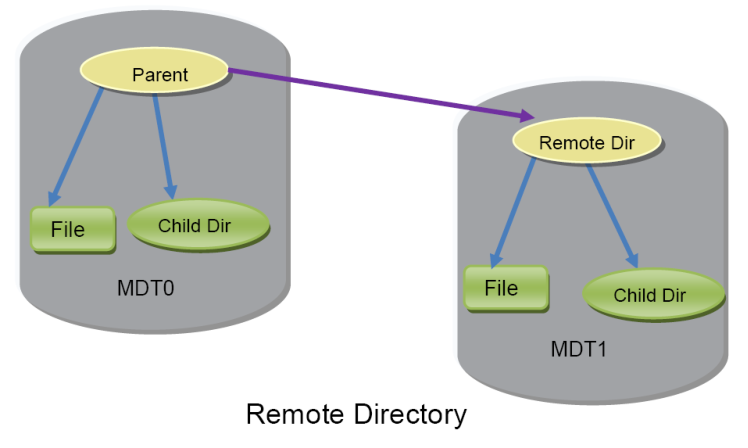
\includegraphics[width=0.5\textwidth]{figs/dnep1}
  \caption{DNE P1 Remote Directories (Courtesy of OpenSFS)}
\end{figure}
 
DNE P2 will provide Lustre the capability to create striped directory in a
similar fashion as bulk I/O is distributed across OSTs. The OSS bulk I/O
packets are distributed in a round robin fashion with applied weights to help
keep OST usage nearly the same across the namespace. In the case of meta data
the distribution is based on a hash calculated for the file in interest. You
can control the hashing done for a striped directory with \code{lfs setdirstripe}
using the \code{–t} or \code{--hash-type} option. Currently only two options are available,
\code{all\_char} which is sum of ASCII characters modulo number of MDTs, or \code{fnv\_1a\_64}
that is the \code{Fowler-Noll-Vo (FNV-1a)} algorithm. From the previous example you
can see the user interface has moved from DNE P1 \code{lfs mkdir} to using
\code{lfs setdirstripe}  for DNE P2. Much like DNE P1 directories creation can
be limited to personnel with root privileges. By default, only directories on
the very first MDT can contain directories that are not on the same MDT. Figure
2 illustrates this Lustre striped directory concept, where a striped directory
is defined as the contents of a given directory are distributed over multiple
MDTs.  Looking back to Figure 1 you will see a similar limitation with DNE P1
in which data from the root remote directory is cached on the first MDT.  

\begin{figure}[!ht]
  \centering
    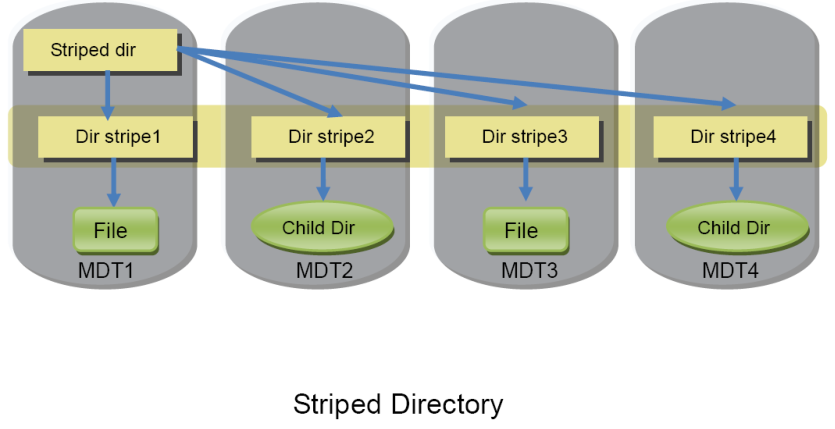
\includegraphics[width=0.5\textwidth]{figs/dnep2}
  \caption{DNE P2 Remote Directories (Courtesy of OpenSFS)}
\end{figure}

In either case we can see the limitation is that MDT1 contains a
disproportionate amount of data. In my testing when the file and directory
count reached high enough the first MDT filled rapidly. Especial in my case the
first MDT was the smallest in my test cluster. For DNE P2 it is possible to
create remote directories with its parent directory located place on any MDT
when you enable \code{remote\_dir}. This can be done by issuing the follow command:

\code{lctl set\_param mdt.*.enable\_remote\_dir=1}

to all available MDS servers. Another feature available in DNE P2 is the
ability to allow non root users to create remote directories. Currently you can
use the default setup up only root or you allow a single specific group to
create a remote directory which handles the case of specific non root
administrative accounts. Lastly you can allow all groups. The way to manage
this feature is by issuing the following command to all MDS servers:

\code{lct set\_param mdt.*.enable\_remote\_dir\_gid=``group\_id''} 

To allow any user to create remove directories set \code{``group\_id''} to \code{-1}. So far all
the functionality discussed has pertained specifically to DNE2. More
functionality exist to the \code{lfs setdirstripe} which was modeled after the same
functionality seen with \code{lfs setstripe}; which is used to manage I/O bulk data
placement on the OSS servers. This was to done to make it easy for new users to
learn quickly this tool since they are already familiar with \code{lfs getstripe}. The
\code{lfs setdirstripe} like its counter part allows setting the striping count and
striping index. The striping index can be used to control which MDT to be first
use to store meta data information. This is most helpful in the case to avoid
MDTs that lack enough disk space. The stripe count determines how many MDTs
will be used to store the file's meta data for a remote directory. Lastly like
a \code{-D} option is available to \code{lfs setdirstripe} to allow the inheritance of the
remote directories configuration.




\subsection{DNE P1 Evaluation}

Our test environment consisted Arthur, which is a single Cray XK7 cabinet with
XYZ nodes. Arthur at the time of DNE P1 tests were running Cray CLE 5.2.UP02
operating system. The Lustre version on clients was 2.5.3. 16 separate x86\_64
systems were configured as Lustre MDS nodes. Servers were running Lustre
version 2.5.3. Each node had a single Toshiba MBF2600RC Serial Attached SCSI
SSD device. These were configured as MDTs, one per MDS.  We used an in-house
modified version of the mdtest benchmark version 1.8.3. Our modification
allowed mdtest to use pre-created directories, which was essential in testing
the DNE P1. In the standard mdtest each iteration of test creates a new
directory \code{test-dir}.The \code{`iteration'} which will always be the non-DNE case. To work
around this case mdtest was modified to use detect the already existing test
directories. The second change is mdtest runs it test against each test
directory one at  a time but since each directory is located on a single MDT
with each being on a different server we can not evaluate the performance gain
in that setup. So the second modification to mdtest was to allow running all
test directory iterations at the same time in parallel. The mdtest benchmark
execution script can be found in Appendix A. The modified mdtest source code
changes will be merged back into the publicly available mdtest soon.


For DNE P1 testing, we used 1,000 files per directory as a constant MDS
directory load. Tests were carried out on October 2014. We used 19 client nodes
on Arthur with 32 tasks per each, 608 tasks total for the tests. Each test were
repeated for 10 iterations. A test sample output is given below:

\begin{lstlisting}

-- started at 10/21/2014 14:22:23 --
mdtest-1.8.3 was launched with 608 total task(s) 
on 19 nodes
Command line used: /lustre/sultan/stf008/scratch
/jsimmons/mdtest -i 10 -I 1000 -v -u -d /lustre
/sultan/stf008/scratch/jsimmons/test_mdt0@
/lustre/sultan/stf008/scratch/jsimmons/test_mdt1
Path: /lustre/sultan/stf008/scratch/jsimmons
FS: 797.1 TiB   Used FS: 0.0%   Inodes: 398.7 Mi
   Used Inodes: 0.0%
608 tasks, 608000 files/directories

Operation               Duration              Rate
   ---------               --------              ----
 * iteration 1 *
   Tree creation     :      0.021 sec,     46.915 ops/sec
   Directory creation:     50.762 sec,  11977.446 ops/sec
   Directory stat    :      5.075 sec, 119803.236 ops/sec
   Directory removal :     17.270 sec,  35206.154 ops/sec
   File creation     :     18.693 sec,  32525.254 ops/sec
   File stat         :     23.776 sec,  25571.721 ops/sec
   File removal      :     38.891 sec,  15633.324 ops/sec
   Tree removal      :      0.053 sec,     18.905 ops/sec
 * iteration 2 *
   Tree creation     :      0.016 sec,     63.646 ops/sec
   Directory creation:     53.253 sec,  11417.247 ops/sec
   Directory stat    :      4.995 sec, 121719.575 ops/sec
   Directory removal :     18.486 sec,  32890.048 ops/sec
   File creation     :     16.301 sec,  37297.574 ops/sec
   File stat         :     23.698 sec,  25656.142 ops/sec
   File removal      :     37.839 sec,  16067.906 ops/sec
   Tree removal      :      0.103 sec,      9.747 ops/sec
 * iteration 3 *
   Tree creation     :      0.048 sec,     20.784 ops/sec
   Directory creation:     56.738 sec,  10715.979 ops/sec
   Directory stat    :      5.006 sec, 121445.960 ops/sec
   Directory removal :     16.371 sec,  37137.929 ops/sec
   File creation     :     22.764 sec,  26708.523 ops/sec
   File stat         :     23.661 sec,  25696.630 ops/sec
   File removal      :     36.232 sec,  16780.610 ops/sec
   Tree removal      :      0.086 sec,     11.603 ops/sec
 * iteration 4 *
   Tree creation     :      0.030 sec,     33.109 ops/sec
   Directory creation:     65.516 sec,   9280.225 ops/sec
   Directory stat    :      5.034 sec, 120789.771 ops/sec
   Directory removal :     10.381 sec,  58570.283 ops/sec
   File creation     :     31.259 sec,  19450.693 ops/sec
   File stat         :     23.761 sec,  25587.876 ops/sec
   File removal      :     37.799 sec,  16085.099 ops/sec
   Tree removal      :      0.092 sec,     10.826 ops/sec
 * iteration 5 *
   Tree creation     :      0.126 sec,      7.917 ops/sec
   Directory creation:     56.259 sec,  10807.185 ops/sec
   Directory stat    :      4.988 sec, 121891.029 ops/sec
   Directory removal :     14.342 sec,  42393.831 ops/sec
   File creation     :     19.169 sec,  31717.449 ops/sec
   File stat         :     23.509 sec,  25862.805 ops/sec
   File removal      :     38.008 sec,  15996.705 ops/sec
   Tree removal      :      0.100 sec,      9.985 ops/sec
 * iteration 6 *
   Tree creation     :      0.024 sec,     41.264 ops/sec
   Directory creation:     50.711 sec,  11989.447 ops/sec
   Directory stat    :      5.050 sec, 120398.587 ops/sec
   Directory removal :     13.716 sec,  44327.294 ops/sec
   File creation     :     23.142 sec,  26272.491 ops/sec
   File stat         :     22.998 sec,  26437.275 ops/sec
   File removal      :     31.862 sec,  19082.082 ops/sec
   Tree removal      :      8.808 sec,      0.114 ops/sec
 * iteration 7 *
   Tree creation     :      0.023 sec,     44.131 ops/sec
   Directory creation:     49.275 sec,  12338.823 ops/sec
   Directory stat    :      4.956 sec, 122684.801 ops/sec
   Directory removal :     17.558 sec,  34627.587 ops/sec
   File creation     :     17.538 sec,  34667.561 ops/sec
   File stat         :     23.453 sec,  25924.256 ops/sec
   File removal      :     38.894 sec,  15632.386 ops/sec
   Tree removal      :      0.071 sec,     14.008 ops/sec
 * iteration 8 *
   Tree creation     :      0.027 sec,     37.594 ops/sec
   Directory creation:     54.556 sec,  11144.496 ops/sec
   Directory stat    :      5.004 sec, 121512.774 ops/sec
   Directory removal :     11.720 sec,  51878.271 ops/sec
   File creation     :     18.477 sec,  32905.459 ops/sec
   File stat         :     24.315 sec,  25005.094 ops/sec
   File removal      :     44.397 sec,  13694.737 ops/sec
   Tree removal      :      0.134 sec,      7.488 ops/sec
 * iteration 9 *
   Tree creation     :      0.027 sec,     37.394 ops/sec
   Directory creation:     53.182 sec,  11432.347 ops/sec
   Directory stat    :      5.063 sec, 120084.463 ops/sec
   Directory removal :     17.930 sec,  33910.568 ops/sec
   File creation     :     24.783 sec,  24532.989 ops/sec
   File stat         :     23.972 sec,  25363.104 ops/sec
   File removal      :     36.834 sec,  16506.375 ops/sec
   Tree removal      :      0.063 sec,     15.902 ops/sec
 * iteration 10 *
   Tree creation     :      0.018 sec,     57.077 ops/sec
   Directory creation:     59.193 sec,  10271.559 ops/sec
   Directory stat    :      5.028 sec, 120923.844 ops/sec
   Directory removal :     16.536 sec,  36768.123 ops/sec
   File creation     :     24.106 sec,  25222.394 ops/sec
   File stat         :     23.863 sec,  25478.979 ops/sec
   File removal      :     39.525 sec,  15382.738 ops/sec
   Tree removal      :      0.049 sec,     20.433 ops/sec

SUMMARY: (of 10 iterations)
   Operation                  Max        Min       Mean    Std Dev
   ---------                  ---        ---       ----    -------
   Directory creation:  12349.796   9283.845  11145.773    869.879
   Directory stat    : 123904.353 120985.660 122593.489    887.006
   Directory removal :  58571.575  32890.567  40771.867   8140.125
   File creation     :  37338.848  19460.639  29148.300   5243.593
   File stat         :  26506.056  25039.761  25720.620    360.899
   File removal      :  19082.413  13694.820  16086.342   1275.494
   Tree creation     :     63.646      7.917     38.983     15.380
   Tree removal      :     20.433      0.114     11.901      5.570

-- finished at 10/21/2014 14:49:01 --
Application 183 resources: utime ~174191s, stime ~9984s, 
Rss ~8752, inblocks ~123436, outblocks ~259931
\end{lstlisting}

Figure 3 shows DNE P1 testing for directory IOPs rates with respect to
increasing MDS nodes. As can be seen, directory deletions quadruple the
performance from 1 to 5 MDS nodes, then the performance drops around 25% and
stays flat. For directory stat operations, the performance gain quickly
diminishes after 3 MDS nodes. For directory create operations, the ramp up is
quite slow compared to deletions and stats, and best performance is obtained at
13 MDS nodes. From these results, OLCF determined that the best deployment
options were to limit the number of MDS nodes to four, if directory operation
rates were the primary performance concern.


\begin{figure}[!ht]
  \centering
    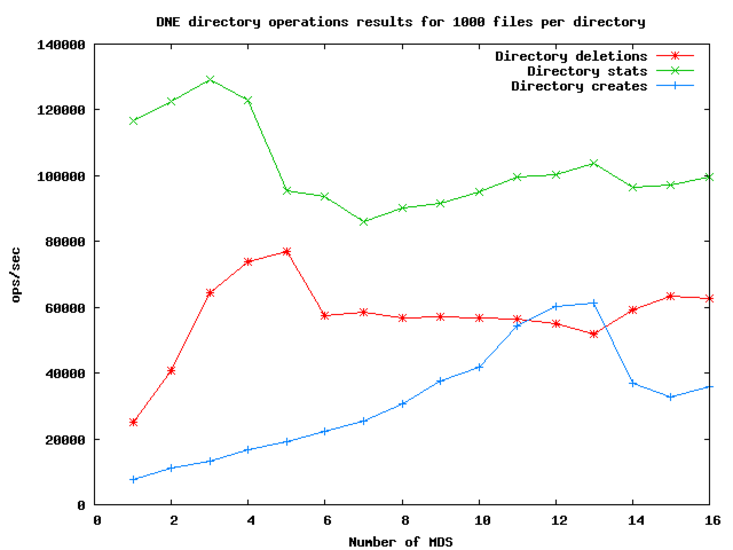
\includegraphics[width=0.5\textwidth]{figs/dnep1_dir_results}
  \caption{DNE P1 directory test results}
\end{figure}


Figure 4 shows our DNE P1 test results with file operations. As can be seen,
file deletion operations scale up nicely up to 15 MDS nodes, where increasing
number of MDS nodes hurts file stat operation rates. File creation performance
doubles up until five MDS nodes only.  Combining DNE P1 test results for
directory and file operations, best rule of thumb was determined as 4 MDS nodes
per namespace for production deployments.


\begin{figure}[!ht]
  \centering
    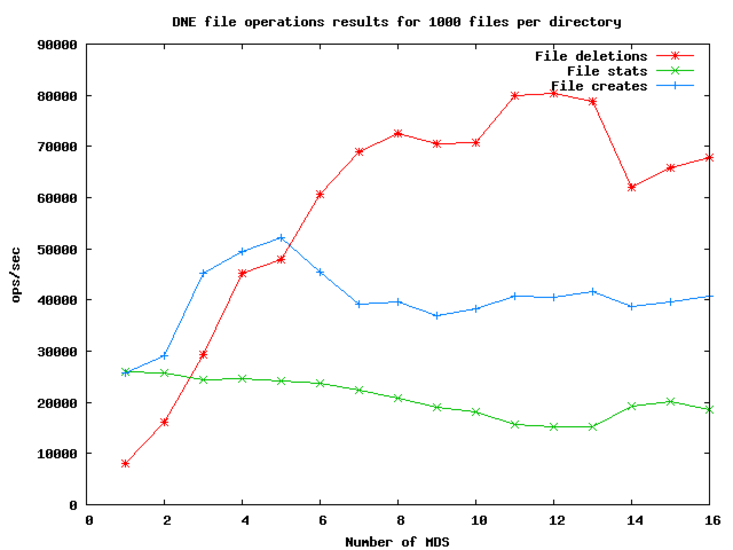
\includegraphics[width=0.5\textwidth]{figs/dnep1_file_results}
  \caption{DNE P1 file test results}
\end{figure}
 


\subsection{DNE P2}

Our test environment consisted Arthur, which is a single Cray XK7 cabinet with
XYZ nodes. Arthur at the time of DNE P2 tests were running Cray CLE 5.2.UP02
operating system. The Lustre version on clients was a specially built pre 2.8
client with a constant evolving patch set. Sixteen separate x86\_64 systems were
configured as Lustre MDS nodes. Servers were running the same Lustre pre 2.8
version as the clients. Each node had a single Toshiba MBF2600RC Serial
Attached SCSI SSD device. These were configured as MDTs, one per MDS. 

We used the same in-house modified version of the mdtest benchmark version
1.8.3. Our modification allowed mdtest to use pre-created directories, which was
essential in testing the DNE P1. The mdtest benchmark execution script can be
found in Appendix A. The modified mdtest source code will be publicly available
soon.

For DNE P2 testing, we used 1,000 files per directory as a constant MDS
directory load. Tests were carried out on October 2014. We used 19 client nodes
on Arthur with 32 tasks per each, 608 tasks total for the tests. Each test were
repeated for 10 iterations.


\section{Production Deployment}

This report has focused mainly on the software side of the DNE Phase 2 roll-out,
however it is important to understand the OLCF's considerations for the
hardware side of this upgrade. We currently have a single metadata server per
Atlas file system. The plan for production is to increase to four metadata
servers per Atlas file system (eight total). Our current production metadata
nodes (MDS nodes) are dual-socket six-core Intel Sandy Bridge 2.5 GHz servers
each with 256GB DDR3 RAM distributed evenly between the two processors, a
single port FDR InfiniBand card, and a dual port 6Gb/s SAS card. Due to the
limited abilities for SMP scaling in the Lustre MDS code and the added NUMA
latency of having the IB card, SAS card, and Lustre MDS processes potentially
living on different CPUs we decided to rethink our approach to building MDS
servers.

The new systems will have a single socket eight-core Intel Haswell 3.2GHz
processor, 256GB DDR RAM, a single port FDR InfiniBand card, and a dual port
12Gb/s SAS card. The new single-socket MDS nodes should reduce NUMA induced
latency, the faster CPU frequency should increase responsiveness from the MDT
threads (due to limited SMP scaling), and the faster SAS link to disk storage
should also increase the performance for flushes (syncs) from MDS memory to the
backend storage.

As part of the process of moving to new hardware, we are also making an
investment in a new backend storage system to store the metadata on. The two
production systems in place currently share a NetApp E5500 storage array
composed of 48 900GB SAS drives with a 6Gb/s interconnect to the MDS nodes. For
the upgrade, we are installing two NetApp EF560 storage arrays each with 24x
1.6TB solid state drives (one storage array per file system), and 12Gb/sec SAS
for host connectivity. Even though most of our metadata operations are in
memory on the MDS nodes, we felt that having 8 MDS servers on a single NetApp
E5500 would be a bottleneck due to the limited IOP throughput of SAS disks. The
NetApp EF560 all solid-state disk solution has provided over 30x improvement in
IOPs at the block level.

\section{Hardware Evaluation for Production Deployment}

We had to make many considerations in measuring the performance of the updated
code. Lustre metadata is written 4 kB out a time assuming that you are not
using a kernel I/O scheduler, which we do not recommend. These small IO size
lends itself to do very well with flash based storage because of the lower
latency and higher IOPs.

In our evaluation of the new storage system we had to conduct tests at the
block level and the Lustre level. How you test the block level depends heavily
on the feature set of the storage hardware. In the case of the NetApp EF560, we
tested read/write performance for all of the following scenarios:

\begin{itemize}

\item Varying I/O segment sizes (32 kB, 64 kB, 128 kB, 256 kB, and 512 kB)

\item Enabling/disabling the DA (data assurance) feature

\item Testing RAID 10 volume groups of varying number of disks (since some RAID subsystems do not handle large RAID volume group performance well)

\item Using a parity decoupled disk volume instead of a RAID10

\item Testing performance from a single node and from all 4 nodes attached to each disk system.

\end{itemize}

To test the block level IO performance we used a tool developed at the OLCF
called fair-lio. It creates a random 4 kB workload, and very effectively
stresses out the disks system. Block-level tests are ongoing at the time of
writing this document. It will be updated will new results in the near future.
After qualifying the performance of the block level performance we will
evaluate the performance at the Lustre software layer. To do this we will
create a small Lustre file system using the new metadata servers and new NetApp
EF560 storage system as the metadata target. We will use the mdtest benchmark
tool for these tests. File system level tests are not complete at the time of
writing this document and it will be updated will new results in the near
future.

\section*{Appendix}

Sarp: This is probably not needed but I am making a dump from the tech report, and I am keeping this for the time being for the sake of completeness. Feel free to knock this one down.

Mdtest script

\begin{verbatim}[fontsize=\small]
#!/bin/bash
#PBS -l nodes=20
#PBS -l walltime=24:00:00
#PBS -N results-mdtest-scale
#PBS -j oe

MOUNT=<filsystem-name>
OSTCOUNT=$(lctl get_param -n lov.$MOUNT-clilov*.numobd)
ITER=5

PBS_JOBID="dne2_8_mds"
BINDIR=/lustre/$MOUNT/$USER
OUTDIR=$BINDIR/${PBS_JOBID}_md_test
[ -e $OUTDIR ] || {
	mkdir -p $OUTDIR
	lfs setstripe -c $OSTCOUNT $OUTDIR
}
cd $BINDIR

#for filecount in 10000 100000 1000000 10000000
for filecount in 1000000 10000000
do
	TOTAL=$(($filecount / 1000))

	for threads in 1 $(seq 5 5 400)
	do
		nodes=$(((threads + 19) / 20))
		[ $nodes -gt 20 ] && nodes=20

		aprun -n $threads -N $nodes $BINDIR/mdtest -I $(( $filecount / $threads)) -i $ITER -d $OUTDIR/shared_${TOTAL}k_$threads
	done

	#for threads in 1 $(seq 5 5 400)
	#do
	#	nodes=$(((threads + 19) / 20))
	#	[ $nodes -gt 20 ] && nodes=20

	#	aprun -n $threads -N $nodes $BINDIR/mdtest -I $(( $filecount / $threads)) -i $ITER -u  -d $OUTDIR/unique_${TOTAL}k_$threads
	#done
done
\end{verbatim}


\section{Conclusions \& Future Work}

Our results generally match expectations, which is good.

% conference papers do not normally have an appendix

% use section* for acknowledgment
\ifCLASSOPTIONcompsoc
  % The Computer Society usually uses the plural form
  \section*{Acknowledgments}
\else
  % regular IEEE prefers the singular form
  \section*{Acknowledgment}
\fi

This work used resources of the Extreme Scale Systems Center, supported
by the Department of Defense, and the Oak Ridge Leadership Computing
Facility, supported by the Office of Science of the Department of
Energy, at Oak Ridge National Laboratory.

Ack Hyperion too.

% trigger a \newpage just before the given reference
% number - used to balance the columns on the last page
% adjust value as needed - may need to be readjusted if
% the document is modified later
%\IEEEtriggeratref{8}
% The "triggered" command can be changed if desired:
%\IEEEtriggercmd{\enlargethispage{-5in}}

% references section

% can use a bibliography generated by BibTeX as a .bbl file
% BibTeX documentation can be easily obtained at:
% http://www.ctan.org/tex-archive/biblio/bibtex/contrib/doc/
% The IEEEtran BibTeX style support page is at:
% http://www.michaelshell.org/tex/ieeetran/bibtex/
%\bibliographystyle{IEEEtran}
% argument is your BibTeX string definitions and bibliography database(s)
%\bibliography{IEEEabrv,../bib/paper}
%
% <OR> manually copy in the resultant .bbl file
% set second argument of \begin to the number of references
% (used to reserve space for the reference number labels box)
\begin{thebibliography}{1}


\bibitem{ior}
"chaos/ior - Parallel filesystem I/O benchmark", \texttt{https://github.com/chaos/ior}.

\bibitem{synthetic-pfl}
Joel Reed et al., "Evaluating Dynamic File Striping for Lustre", \emph{International Workshop on the Lustre Ecosystem: Challenges and Opportunities}, March 2015.

\bibitem{sarp-cug}
Sarp Oral et al., "OLCF`s 1TB$/$s, Next-Generation Lustre File System", \emph{Cray User Group 2013}, May 2013.

\bibitem{dne-contract}
"OpenSFS DNE Contract", \texttt{http://wiki.opensfs.org/Contract\_SFS-DEV-001}.

\end{thebibliography}


% that's all folks
\end{document}


